%% abtex2-modelo-relatorio-tecnico.tex, v<VERSION> laurocesar
%% Copyright 2012-<COPYRIGHT_YEAR> by abnTeX2 group at http://www.abntex.net.br/ 
%%
%% This work may be distributed and/or modified under the
%% conditions of the LaTeX Project Public License, either version 1.3
%% of this license or (at your option) any later version.
%% The latest version of this license is in
%%   http://www.latex-project.org/lppl.txt
%% and version 1.3 or later is part of all distributions of LaTeX
%% version 2005/12/01 or later.
%%
%% This work has the LPPL maintenance status `maintained'.
%% 
%% The Current Maintainer of this work is the abnTeX2 team, led
%% by Lauro César Araujo. Further information are available on 
%% http://www.abntex.net.br/
%%
%% This work consists of the files abntex2-modelo-relatorio-tecnico.tex,
%% abntex2-modelo-include-comandos and abntex2-modelo-references.bib
%%

% ------------------------------------------------------------------------
% ------------------------------------------------------------------------
% abnTeX2: Modelo de Relatório Técnico/Acadêmico em conformidade com 
% ABNT NBR 10719:2015 Informação e documentação - Relatório técnico e/ou
% científico - Apresentação
% ------------------------------------------------------------------------ 
% ------------------------------------------------------------------------

\documentclass[
% -- opções da classe memoir --
12pt,				% tamanho da fonte
openany,			% capítulos começam em pág ímpar (insere página vazia caso preciso)
twoside,			% para impressão em recto e verso. Oposto a oneside
a4paper,			% tamanho do papel. 
% -- opções da classe abntex2 --
%chapter=TITLE,		% títulos de capítulos convertidos em letras maiúsculas
%section=TITLE,		% títulos de seções convertidos em letras maiúsculas
%subsection=TITLE,	% títulos de subseções convertidos em letras maiúsculas
%subsubsection=TITLE,% títulos de subsubseções convertidos em letras maiúsculas
% -- opções do pacote babel --
english,			% idioma adicional para hifenização
french,				% idioma adicional para hifenização
spanish,			% idioma adicional para hifenização
brazil,				% o último idioma é o principal do documento
]{abntex2}


% ---
% PACOTES
% ---

% ---
% Pacotes fundamentais 
% ---
\usepackage{lmodern}			% Usa a fonte Latin Modern
\usepackage[T1]{fontenc}		% Selecao de codigos de fonte.
\usepackage[utf8]{inputenc}		% Codificacao do documento (conversão automática dos acentos)
\usepackage{indentfirst}		% Indenta o primeiro parágrafo de cada seção.
\usepackage{color}				% Controle das cores
\usepackage{graphicx}			% Inclusão de gráficos
\usepackage{microtype} 			% para melhorias de justificação
% ---

% ---
% Pacotes adicionais, usados no anexo do modelo de folha de identificação
% ---
\usepackage{multicol}
\usepackage{multirow}
% ---

% ---
% Pacotes adicionais, usados apenas no âmbito do Modelo Canônico do abnteX2
% ---
\usepackage{lipsum}				% para geração de dummy text
% ---

% ---
% Pacotes de citações
% ---
\usepackage[brazilian,hyperpageref]{backref}	 % Paginas com as citações na bibl
\usepackage[alf]{abntex2cite}	% Citações padrão ABNT

% ---
% Pacotes pessoais
% ---


\definecolor{mygreen}{rgb}{0,0.6,0}
\definecolor{mygray}{rgb}{0.5,0.5,0.5}
\definecolor{mymauve}{rgb}{0.58,0,0.82}
\definecolor{bege}{rgb}{0.95,0.95,0.9}

\usepackage{caption}

\usepackage{listings}				% para inclusão de códigos-fonte no documento
\lstdefinestyle{bash}{ 
    backgroundcolor=\color{black},   % choose the background color; you must add \usepackage{color} or \usepackage{xcolor}; should come as last argument
    basicstyle=\footnotesize\color{white},        % the size of the fonts that are used for the code
    breakatwhitespace=false,         % sets if automatic breaks should only happen at whitespace
    breaklines=true,                 % sets automatic line breaking
    captionpos=b,                    % sets the caption-position to bottom
    commentstyle=\color{red},    % comment style
    deletekeywords={...},            % if you want to delete keywords from the given language
    escapeinside={\%*}{*)},          % if you want to add LaTeX within your code
    extendedchars=true,              % lets you use non-ASCII characters; for 8-bits encodings only, does not work with UTF-8
    keepspaces=true,                 % keeps spaces in text, useful for keeping indentation of code (possibly needs columns=flexible)
    columns=flexible,                 % keeps spaces in text, useful for keeping indentation of code (possibly needs columns=flexible)
    keywordstyle=\color{green},       % keyword style
    language=bash,                  % the language of the code
    linecolor=\color{black},
    morekeywords={*,..., sudo, curl},            % if you want to add more keywords to the set
    numbers=left,                    % where to put the line-numbers; possible values are (none, left, right)
    numbersep=5pt,                   % how far the line-numbers are from the code
    numberstyle=\tiny\color{mygray}, % the style that is used for the line-numbers
    rulecolor=\color{black},         % if not set, the frame-color may be changed on line-breaks within not-black text (e.g. comments (green here))
    showspaces=false,                % show spaces everywhere adding particular underscores; it overrides 'showstringspaces'
    showstringspaces=false,          % underline spaces within strings only
    showtabs=false,                  % show tabs within strings adding particular underscores
    stepnumber=1,                    % the step between two line-numbers. If it's 1, each line will be numbered
    stringstyle=\color{yellow},     % string literal style
    tabsize=2,                       % sets default tabsize to 2 spaces
    title=\lstname                   % show the filename of files included with \lstinputlisting; also try caption instead of title
}


\lstdefinestyle{php}{ 
    backgroundcolor=\color{black},   % choose the background color; you must add \usepackage{color} or \usepackage{xcolor}; should come as last argument
    basicstyle=\footnotesize\color{white},        % the size of the fonts that are used for the code
    breakatwhitespace=false,         % sets if automatic breaks should only happen at whitespace
    breaklines=true,                 % sets automatic line breaking
    captionpos=b,                    % sets the caption-position to bottom
    commentstyle=\color{red},    % comment style
    deletekeywords={...},            % if you want to delete keywords from the given language
    escapeinside={\%*}{*)},          % if you want to add LaTeX within your code
    extendedchars=true,              % lets you use non-ASCII characters; for 8-bits encodings only, does not work with UTF-8
    keepspaces=true,                 % keeps spaces in text, useful for keeping indentation of code (possibly needs columns=flexible)
    columns=flexible,                 % keeps spaces in text, useful for keeping indentation of code (possibly needs columns=flexible)
    keywordstyle=\color{green},       % keyword style
    language=php,                  % the language of the code
    linecolor=\color{black},
    morekeywords={*,..., class, extends, protected, public, private, function},            % if you want to add more keywords to the set
    numbers=left,                    % where to put the line-numbers; possible values are (none, left, right)
    numbersep=5pt,                   % how far the line-numbers are from the code
    numberstyle=\tiny\color{mygray}, % the style that is used for the line-numbers
    rulecolor=\color{black},         % if not set, the frame-color may be changed on line-breaks within not-black text (e.g. comments (green here))
    showspaces=false,                % show spaces everywhere adding particular underscores; it overrides 'showstringspaces'
    showstringspaces=false,          % underline spaces within strings only
    showtabs=false,                  % show tabs within strings adding particular underscores
    stepnumber=1,                    % the step between two line-numbers. If it's 1, each line will be numbered
    stringstyle=\color{yellow},     % string literal style
    tabsize=2,                       % sets default tabsize to 2 spaces
    title=\lstname                   % show the filename of files included with \lstinputlisting; also try caption instead of title
}


\lstdefinestyle{common}{ 
    backgroundcolor=\color{bege},   % choose the background color; you must add \usepackage{color} or \usepackage{xcolor}; should come as last argument
    basicstyle=\color{black},        % the size of the fonts that are used for the code
    breakatwhitespace=false,         % sets if automatic breaks should only happen at whitespace
    breaklines=true,                 % sets automatic line breaking
    captionpos=b,                    % sets the caption-position to bottom
    commentstyle=\color{red},    % comment style
    deletekeywords={...},            % if you want to delete keywords from the given language
    escapeinside={\%*}{*)},          % if you want to add LaTeX within your code
    extendedchars=true,              % lets you use non-ASCII characters; for 8-bits encodings only, does not work with UTF-8
    keepspaces=true,                 % keeps spaces in text, useful for keeping indentation of code (possibly needs columns=flexible)
    columns=flexible,                 % keeps spaces in text, useful for keeping indentation of code (possibly needs columns=flexible)
    keywordstyle=\color{mygreen},       % keyword style
    language=php,                  % the language of the code
    linecolor=\color{black},
    morekeywords={*,..., class, extends, protected, public, private, function},            % if you want to add more keywords to the set
    numbers=none,                    % where to put the line-numbers; possible values are (none, left, right)
    numbersep=5pt,                   % how far the line-numbers are from the code
    numberstyle=\tiny\color{mygray}, % the style that is used for the line-numbers
    rulecolor=\color{black},         % if not set, the frame-color may be changed on line-breaks within not-black text (e.g. comments (green here))
    showspaces=false,                % show spaces everywhere adding particular underscores; it overrides 'showstringspaces'
    showstringspaces=false,          % underline spaces within strings only
    showtabs=false,                  % show tabs within strings adding particular underscores
    stepnumber=1,                    % the step between two line-numbers. If it's 1, each line will be numbered
    stringstyle=\color{blue},     % string literal style
    tabsize=2,                       % sets default tabsize to 2 spaces
    title=\lstname                   % show the filename of files included with \lstinputlisting; also try caption instead of title
}

\lstdefinestyle{c}{
    language=C++,
    basicstyle=\ttfamily\footnotesize, 
    keywordstyle=\color{blue}, 
    stringstyle=\color{x}, 
    commentstyle=\color{red}, 
    extendedchars=true, 
    showspaces=false, 
    showstringspaces=false, 
    %numbers=left,
    % numberstyle=\tiny,
    breaklines=true, 
    backgroundcolor=\color{gray!10},
    breakautoindent=true, 
    captionpos=t,
    xleftmargin=0pt,
}

\usepackage{tcolorbox}      % Para box arredondado
\usepackage{tabularx}
\usepackage{array}
\usepackage{colortbl}
\usepackage{float}      % para usar o H como parâmetro no include figure
% ---

% --- 
% CONFIGURAÇÕES DE PACOTES
% --- 
\renewcommand{\labelitemi}{}
% ---
% Configurações do pacote backref
% Usado sem a opção hyperpageref de backref
\renewcommand{\backrefpagesname}{Citado na(s) página(s):~}
% Texto padrão antes do número das páginas
\renewcommand{\backref}{}
% Define os textos da citação
\renewcommand*{\backrefalt}[4]{
    \ifcase #1 %
        Nenhuma citação no texto.%
        \or
        Citado na página #2.%
    \else
        Citado #1 vezes nas páginas #2.%
\fi}%
% ---

% ---
% Informações de dados para CAPA e FOLHA DE ROSTO
% ---
\titulo{Central de controle em domótica via Internet}
\autor{Gabriel Marques de Melo}
\local{Brasil}
\data{2018}
\instituicao{%
    Universidade Federal de Lavras
    \par
    Departamento de Engenharia
    \par
Graduação em Ciência da Computação}

\tipotrabalho{Relatório técnico}
% O preambulo deve conter o tipo do trabalho, o objetivo, 
% o nome da instituição e a área de concentração 
\preambulo{Relatório técnico com o objetivo de documentação e apresentação do projeto desenvolvido na Universidade Federal de Lavras, no curso de Ciência da Computação.}
% ---

% ---
% Configurações de aparência do PDF final

% alterando o aspecto da cor azul
\definecolor{blue}{RGB}{41,5,195}

% informações do PDF
\makeatletter
\hypersetup{
    %pagebackref=true,
    pdftitle={\@title}, 
    pdfauthor={\@author},
    pdfsubject={\imprimirpreambulo},
    pdfcreator={LaTeX with abnTeX2},
    pdfkeywords={abnt}{latex}{abntex}{abntex2}{relatório técnico}, 
    colorlinks=true,       		% false: boxed links; true: colored links
    linkcolor=blue,          	% color of internal links
    citecolor=blue,        		% color of links to bibliography
    filecolor=magenta,      		% color of file links
    urlcolor=blue,
    bookmarksdepth=4
}
\makeatother
% --- 

% --- 
% Espaçamentos entre linhas e parágrafos 
% --- 

% O tamanho do parágrafo é dado por:
\setlength{\parindent}{1.3cm}

% Controle do espaçamento entre um parágrafo e outro:
\setlength{\parskip}{0.2cm}  % tente também \onelineskip

% ---
% compila o indice
% ---
\makeindex
% ---

% ----
% Início do documento
% ----
\begin{document}

% Seleciona o idioma do documento (conforme pacotes do babel)
%\selectlanguage{english}
\selectlanguage{brazil}

% Retira espaço extra obsoleto entre as frases.
\frenchspacing 

% ----------------------------------------------------------
% ELEMENTOS PRÉ-TEXTUAIS
% ----------------------------------------------------------
% \pretextual

% ---
% Capa
% ---
\imprimircapa
% ---

% ---
% Folha de rosto
% (o * indica que haverá a ficha bibliográfica)
% ---
\imprimirfolhaderosto*
% ---

\iffalse
    % ---
    % Anverso da folha de rosto:
    % ---

    {
        \ABNTEXchapterfont

        \vspace*{\fill}

        Conforme a ABNT NBR 10719:2015, seção 4.2.1.1.1, o anverso da folha de rosto
        deve conter:

        \begin{alineas}
        \item nome do órgão ou entidade responsável que solicitou ou gerou o
            relatório; 
        \item título do projeto, programa ou plano que o relatório está relacionado;
        \item título do relatório;
        \item subtítulo, se houver, deve ser precedido de dois pontos, evidenciando a
            sua subordinação ao título. O relatório em vários volumes deve ter um título
            geral. Além deste, cada volume pode ter um título específico; 
        \item número do volume, se houver mais de um, deve constar em cada folha de
            rosto a especificação do respectivo volume, em algarismo arábico; 
        \item código de identificação, se houver, recomenda-se que seja formado
            pela sigla da instituição, indicação da categoria do relatório, data,
            indicação do assunto e número sequencial do relatório na série; 
        \item classificação de segurança. Todos os órgãos, privados ou públicos, que
            desenvolvam pesquisa de interesse nacional de conteúdo sigiloso, devem
            informar a classificação adequada, conforme a legislação em vigor; 
        \item nome do autor ou autor-entidade. O título e a qualificação ou a função
            do autor podem ser incluídos, pois servem para indicar sua autoridade no
            assunto. Caso a instituição que solicitou o relatório seja a mesma que o
            gerou, suprime-se o nome da instituição no campo de autoria; 
        \item local (cidade) da instituição responsável e/ou solicitante; NOTA: No
            caso de cidades homônimas, recomenda-se o acréscimo da sigla da unidade da
            federação.
        \item ano de publicação, de acordo com o calendário universal (gregoriano),
            deve ser apresentado em algarismos arábicos.
        \end{alineas}

        \vspace*{\fill}
    }

    % ---
    % Agradecimentos
    % ---
    \begin{agradecimentos}
        O agradecimento principal é direcionado a Youssef Cherem, autor do
        \nameref{formulado-identificacao} (\autopageref{formulado-identificacao}).

        Os agradecimentos especiais são direcionados ao Centro de Pesquisa em
        Arquitetura da Informação\footnote{\url{http://www.cpai.unb.br/}} da Universidade de
        Brasília (CPAI), ao grupo de usuários
        \emph{latex-br}\footnote{\url{http://groups.google.com/group/latex-br}} e aos
        novos voluntários do grupo
        \emph{\abnTeX}\footnote{\url{http://groups.google.com/group/abntex2} e
        \url{http://www.abntex.net.br/}}~que contribuíram e que ainda
        contribuirão para a evolução do abn\TeX.

    \end{agradecimentos}
\fi
% ---

% ---
% RESUMO
% ---

% resumo na língua vernácula (obrigatório)
\setlength{\absparsep}{18pt} % ajusta o espaçamento dos parágrafos do resumo
\begin{resumo}

    O aprimoramento das comunicações sem fio e o custo cada vez menor de
    dispositivos que se comunicam desta forma, impulsionaram o movimento da
    Internet das coisas bem como as técnicas de acesso remoto via Internet. Neste
    cenário, a domótica, que oferece praticidade, conforto e segurança aos lares,
    ganhou popularidade e foco de pesquisas e projetos. Residências
    automatizadas fornecem controle remoto de dispositivos, como lâmpadas,
    climatizadores e portas, além de informações de monitoramento do lar por
    sensores e câmeras. Nosso projeto, de finalidade aplicada, tem como objetivo
    geral discutir e criar um sistema de controle de automação residencial seguro,
    por acesso remoto via internet, com quantidade de nós atuadores escalável e
    de custo reduzido. A análise quantitativa da escalabilidade e desempenho dos
    nós fornece um parâmetro de comparação em relação às outras modelagens
    empregadas para o problema. Como protótipo, foi desenvolvido um servidor
    web HTTP, para acesso do usuário, utilizando um Raspberry Pi Model B, com
    imagem ubuntu 16.04.1, implementado na linguagem de programação PHP
    7.0.3 e o framework web Laravel 5.5.40. Os nós foram projetados em uma
    placa de circuito impresso que tem como controlador um esp8266-01 e alguns
    atuadores e sensores genéricos. Além da escalabilidade dos nós, estes
    estabelecem uma conexão bidirecional por Web Socket com um servidor em
    Node.js integrado ao mesmo servidor web, comunicando com o sistema em
    tempo real.

    \noindent
    \textbf{Palavras-chaves}: domótica. acesso remoto. servidor web.
\end{resumo}
% ---

% ---
% inserir lista de ilustrações
% ---
\pdfbookmark[0]{\listfigurename}{lof}
\listoffigures*
\cleardoublepage
% ---

% ---
% inserir lista de tabelas
% ---
\pdfbookmark[0]{\listtablename}{lot}
\listoftables*
\cleardoublepage
% ---

% ---
% inserir lista de tabelas
% ---
\pdfbookmark[0]{\listlistings}{lot}
\lstlistoflistings
\cleardoublepage
% ---

% ---
% inserir lista de abreviaturas e siglas
% ---
\begin{siglas}
\item[ABNT] Associação Brasileira de Normas Técnicas
\item[abnTeX] ABsurdas Normas para TeX
\end{siglas}
% ---

% ---
% inserir lista de símbolos
% ---
\begin{simbolos}
\item[$ \Gamma $] Letra grega Gama
\item[$ \Lambda $] Lambda
\item[$ \zeta $] Letra grega minúscula zeta
\item[$ \in $] Pertence
\end{simbolos}
% ---

% ---
% inserir o sumario
% ---
\pdfbookmark[0]{\contentsname}{toc}
\tableofcontents*
\cleardoublepage
% ---


% ----------------------------------------------------------
% ELEMENTOS TEXTUAIS
% ----------------------------------------------------------
\textual

% ----------------------------------------------------------
% Introdução (exemplo de capítulo sem numeração, mas presente no Sumário)
% ----------------------------------------------------------
\chapter*[Introdução]{Introdução}
\addcontentsline{toc}{chapter}{Introdução}
Este documento surgiu com o propósito de documentar as atividades e progressos
realizados durante o período de orientado voluntário, pelo PIVIC, sob orientação
do professor Fabio Domingues de Jesus, do Departamento de Engenharia da UFLA.

Os conteúdos baseados para redação deste estão devidamente referenciados ao final da obra. Considerável parcela
das obras consultadas são de materiais de minha autoria, disponíveis em meu \href{https://github.com/GabrielMMelo/}{github}.

A documentação assume um teor didático, de forma a introduzir novos
orientados ao projeto e que estes, por sua vez, incrementarão o mesmo, 
construindo uma sólida referência do projeto.

O \textbf{referencial teórico} possui um capítulo no estilo \textit{getting started} para cada uma das tecnologias utilizadas. Neste momento, são abordados pontos sobre preparação do ambiente, funcionalidades e exemplos.

Em \textbf{desenvolvimento}, será apresentado o projeto em si. A arquitetura do projeto, bem como os principais trechos de código serão exaltados. 

Os \textbf{resultados} é descrito os valores qualiquantitativos obtidos com o projeto.

E por fim, são sugeridos \textbf{trabalhos futuros} que servirão como incremento, otimização e correção de componentes atuais.

O documento pode servir como ponto de partida para novos projetos correlatos
e sua distribuição deve ser estimulada.

Este documento foi redigido em \LaTeX usando o pacote \textit{abnTeX2}.
% ----------------------------------------------------------
% PARTE - preparação da pesquisa
% ----------------------------------------------------------
\part{Projeto}

% ----------------------------------------------------------
% PARTE - preparação da pesquisa
% ----------------------------------------------------------
\part{Referencial teórico}

% ----------------------------------------------------------
% Capitulo com exemplos de comandos inseridos de arquivo externo 
% ----------------------------------------------------------

%\include{abntex2-modelo-include-comandos}

\section{Placas fotovoltaicas}

\begin{figure}[ht!]
    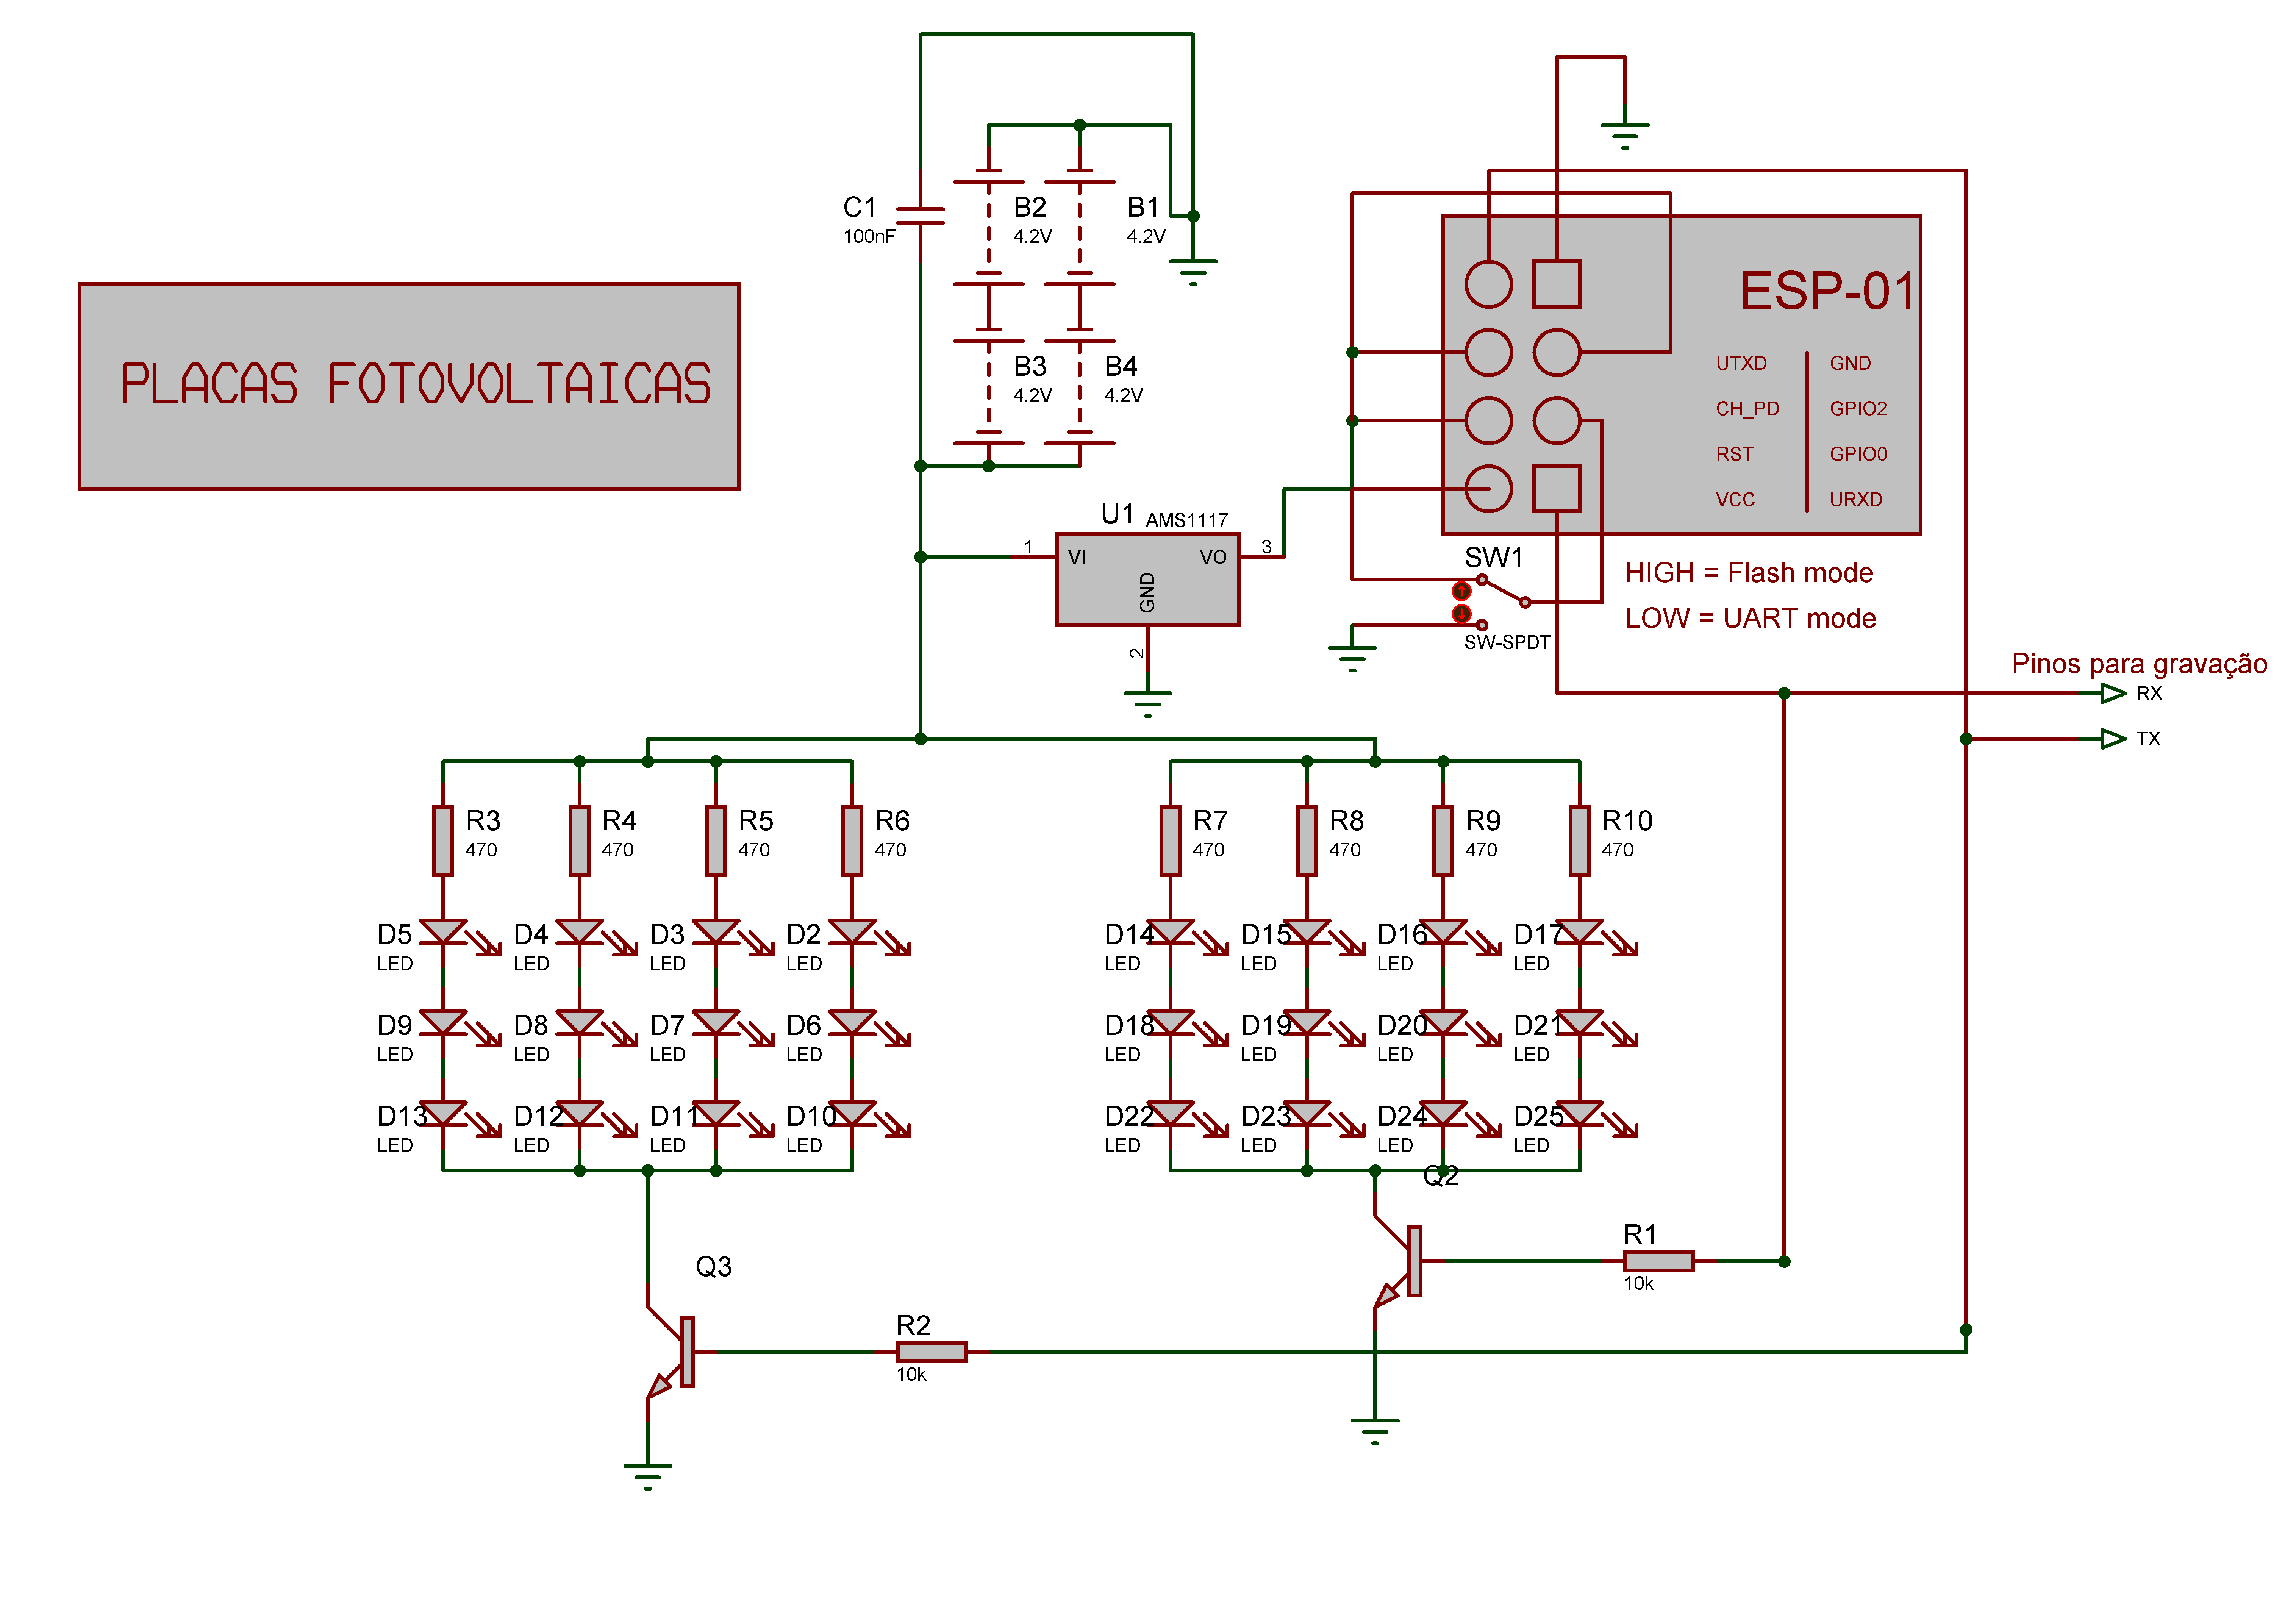
\includegraphics[width=450pt]{images/circuit.png}
    \caption{Foto do protótipo montado}
\end{figure}

\chapter{Esp8266}
É um microcontrolador de 32-bits com modem \textit{Wi-Fi} integrado desenvolvido pela \textit{Espressif Systems}
surgido, em meados de 2014, para suprir a contínua demanda por uma plataforma que fosse de \textsf{\textbf{baixo consumo}} 
energético, \textsf{\textbf{compacta}} e de \textsf{\textbf{desempenho confiável}} na industria de \textit{IoT}.

Assim como a maioria dos modelos Arduino, o ESP possui GPIOs (Pinos de entrada e saída de propósito geral)
e suporte a PWM (Modulação por largura de pulso). O upload do firmware é feito também pela UART (RX/TX), 
porém o ESP8266 conta com upload OTA (over-the-air), que é a gravação através de uma rede.  

Seguir pontos do curso
\section{Especificações}

\subsection{CPU}

O ESP8266 utiliza o processador Tensilica L106 32-bit, RISC e que possui velocidade de clock de 80MHz.
\vspace{10pt} 
\begin{tcolorbox}[colbacktitle=green!50!white!60,
    title={\vspace{-13pt}
\includegraphics[scale=0.032]{images/notebook.png} \hspace{2pt} \textsf{\textbf{Na Prática...}\vspace{4pt}}},coltitle=black, colback=white,arc=4mm, outer arc=3.5mm]
    \raggedright

    Facilmente, podemos alterar - \textit{overclock} - da \textit{CPU} para 160MHz! Para isso, basta adicionarmos o seguinte código no escopo geral do código:
    \begin{lstlisting}[style=c]
    extern "C" {
        bool system_update_cpu_req(int);
        }

    \end{lstlisting}

    E na função \emph{setup()}:
    \begin{lstlisting}[style=c]
    void setup(){
        ...
        system_update_cpu_freq(160);
        ...
    }
    \end{lstlisting}
\end{tcolorbox}

\subsection{Modem \textit{Wi-Fi}}
Com um completo e autônomo sistema de conexão \textit{Wi-Fi} (suporte a \textit{802.11b/g/n/e/i}), o \textit{ESP8266} pode tanto estabelecer uma rede própria, em modo \textbf{\textsf{AP}}, ou um se conectar a um \textit{host}, em modo \textbf{\textsf{STA}}. Possui ainda o modo \textbf{\textsf{AP\_STA}}, que cria uma rede, mas também acessa uma \textit{station}, simultaneamente. 

Pode ser implementado como um "módulo \emph{WiFi}" em conjunto com qualquer microcontrolador e comunicá-los através de interfaces \textbf{\textsf{SPI}}, \textbf{\textsf{I2C}} e \textbf{\textsf{UART}} disponíveis na placa. 

\subsection{Alimentação}

A faixa de tensão de operação do \textit{ESP8266} é de \textbf{\textsf{2.5V}} à \textbf{\textsf{3.6V}}, sendo necessário o fornecimento de, ao menos, \textbf{\textsf{500mA}} de corrente.
\vspace{5pt}

\begin{tcolorbox}[colbacktitle=red!65!white,
    title={\vspace{-13pt}
\includegraphics[scale=0.014]{images/x.png} \hspace{2pt} \textsf{\textbf{CUIDADO!}\vspace{2pt}}},coltitle=black, colback=white,arc=4mm, outer arc=3.5mm]
    \raggedright
    O ESP8266 \textsf{\textbf{não é}} tolerante à 5V. Alimentá-lo com essa tensão pode - \textit{e vai} - danificar seu dispositivo.
\end{tcolorbox}



\subsection{Modos de operação}
O \textit{ESP8266} possui \textbf{\textsf{três}} modos de boot: 

\begin{table}[!ht]
    \centering
    \footnotesize{
        \label{Modos-Energia}
        \caption{Modos de boot}
        \begin{tabular}{>{\bfseries}lp{5.35cm}}
            \toprule
            UART mode & Modo deve ser selecionado para realizar o upload de um novo \textit{firmware} no MCU. A \textbf{\textsf{GPIO0}} deve estar em \textbf{\textsf{GND} / \textbf{\textsf{GPIO2}} em \textbf{\textsf{VCC}}}. \\\midrule
            Flash mode & Neste modo, o boot é realizado da memória \textit{flash}. O último firmware gravado será executado. A \textbf{\textsf{GPIO0}} deve estar em \textbf{\textsf{VCC}} / \textbf{\textsf{GPIO2}} em \textbf{\textsf{VCC}} \\\midrule
            SDIO mode & Quando habilitado, o MCU realiza o boot não da memória \textit{flash}, mas sim de um cartão SD, usando protocolo \textit{SPI}. A \textbf{\textsf{GPIO15}} deve estar em \textbf{\textsf{VCC}}. \\\bottomrule
        \end{tabular}
    }
\end{table}

\subsection{GPIOS}

O \textit{ESP8266} possui 17 pinos GPIO que podem assumir varias funções através da devida programação de seus registradores. Cada um dos pinos pode ser configurado com \textbf{\textsf{pull-up}} ou \textbf{\textsf{pull-down}} interno e também alta impedância. Possui um pino \textbf{\textsf{ADC}}, TOUT $\perp$ 9, de resolução de 1024 bits, porém sua alimentação deve ser limitada de 0 a 1V.

\subsection{\textit{I2C}}
\textit{I2C} (\textit{Inter-integrated Circuit}) é um protocolo de comunicação \textit{master/slave} entre dispositivos que se baseia em um barramento de apenas duas vias: \textbf{\textsf{SDA}} (Serial Data) por onde são transmitidos e recebidos os dados e \textbf{\textsf{SCL}} (Serial Clock) que dita a temporização do tráfego das informações. O grande diferencial do protocolo é que são permitidos, teoricamente, até 127 dispositivos distintos comunicando através de um mesmo barramento.

O ESP8266 possui suporte a interface \textit{I2C}, tanto como Master quanto Slave, para comunicação com outros microcontroladores e outros equipamentos periféricos, como sensores. A pinagem do barramento é vista pela Tabela \ref{I2C-table} abaixo:

\begin{table}[ht]
    \centering
    \caption{Pinagem I2C \label{I2C-table}}
    \begin{tcolorbox}[tabularx={c|Y|Y}]
        \textbf{Pino} & \textbf{Função}     & \textbf{Descrição}    \\\hline
        \emph{GPIO02 $\perp$ 14}      & SDA   & Pino de dados   \\
        \emph{MTMS $\perp$ 9}          & SCL   & Pino de Clock           
    \end{tcolorbox}
\end{table}     

\subsection{UART}

O \textit{ESP8266} possui \textbf{\textsf{duas}} interfaces \textit{UART }(Universal Asynchronous Receiver/Transmitter) que podem alcançar\textbf{ \textsf{4.5 Mbps}} de velocidade de transferência: a \textbf{\textsf{UART0}}, que pode ser usada para comunicação bidirecional; e a \textbf{\textsf{UART1}} que apenas envia dados, por seu pino \textit{TX} (geralmente usado como \textit{debugger}).

\begin{table}[ht]
    \centering
    \caption{Pinagem UART \label{UART-table}}
    \begin{tcolorbox}[tabularx={c |Y|Y}]
    \textbf{Pino} & \textbf{Função}     & \textbf{Descrição}    \\\hline
    \emph{GPIO1 $\perp$ 26}      & TX0   & \small{Transmissão Serial}   \\
    \emph{GPIO3 $\perp$ 25}          & RX0   & \small{Recepção Serial}  \\
    \emph{GPIO2 $\perp$ 23}          & TX1   & \small{Transmissão Serial}          
\end{tcolorbox}
\end{table}     

\subsection{Watchdog}
\textit{Watchdog timer} é um circuito contador independente do clock principal e que serve como um recurso de segurança adicional.

Uma das maiores diferenças entre o \textit{ESP8266} e um MCU utilizado em alguns modelos \textit{Arduino}, é o fato de que o microcontrolador da \textit{Espressif} executa varias tarefas em segundo plano: mantém a conexão do modem Wi-Fi, gerencia a pilha do protocolo TCP/IP, etc. Para manter a execução destas tarefas, ele possui dois watchdog timers: \textbf{\textsf{SW\_WDT}}, que é via software; e \textbf{\textsf{HW\_WDT}}, via Hardware. Caso uma função gere um loop longo (mais de 3 segundos) onde não haja alimentação do watchdog, o microcontrolador irá reiniciar, justamente para manter a execução das tarefas de segundo plano.

Consulte a subseção \ref{subsec:yield-oi} para melhor entendimento de como o software controla o \textit{timer} do \textit{Watchdog}. Este tópico tratará da função \emph{yield()}, que realiza a alimentação do \textbf{\textsf{SW\_WDT}}.

\subsection{PWM}

\textit{PWM} (ou \textit{Modulação por Largura de Pulso}) se refere a um tipo de sinal digital que permite a variação do tempo, de forma analógica, em que um sinal digital assume nível lógico alto. Desta forma, é possível modular a largura do pulso (duração do nível alto) e gerar sinais de tensões intermediárias. 

\vspace{10pt}

\begin{tcolorbox}[colbacktitle=green!50!white!60,
    title={\vspace{-13pt}
\includegraphics[scale=0.032]{images/notebook.png} \hspace{2pt} \textsf{\textbf{Na Prática...}\vspace{4pt}}},coltitle=black, colback=white,arc=4mm, outer arc=3.5mm]
    \raggedright
    Para usarmos um pino como saída de PWM:
    \begin{lstlisting}[style=c]
    analogWrite(pino, valor); 
    \end{lstlisting}
    Alterar a frequência do sinal:
    \begin{lstlisting}[style=c]
    analogWriteFreq(novaFrequencia); //100 Hz and 1 kHz
    \end{lstlisting}
    Alterar o \textit{range} do sinal:
    \begin{lstlisting}[style=c]
    analogWriteRange(novoRange); // 1024 por padrão -> 2^10
    \end{lstlisting}

\end{tcolorbox}

\vspace{7pt}
\begin{tcolorbox}[colbacktitle=blue!70!white!50,
    title={\vspace{-13pt}
\includegraphics[scale=0.033]{images/interrogacao.png} \hspace{2pt} \textsf{\textbf{Você sabia?}\vspace{4pt}}},coltitle=black, colback=white,arc=4mm, outer arc=3.5mm]
    \raggedright

    Uma clássica experiência do modelo pode ser realizada ao chavear, rapidamente, o interruptor da iluminação do seu quarto, por exemplo. A sensação será a de uma iluminação intermediária entre lâmpada desligada e normalmente acesa.

\end{tcolorbox}



O ESP8266 possui 4 pinos de interface \textit{PWM}, mas podem ser estendidos pelo usuário. A definição padrão dos pinos é dada pela Tabela \ref{PWM-table} abaixo.



\begin{table}[ht]
    \centering
    \caption{Pinagem PWM \label{PWM-table}}
    \resizebox{0.5\textheight}{!}{
        \begin{threeparttable}

            \begin{tcolorbox}[tabularx={X|Y}]
                \textbf{Pino} & \textbf{Função}   \\\hline
                \emph{MTDI $\perp$ 10}      & PWM0   \\
                \emph{MTDO $\perp$ 13}          & PWM1  \\
                \emph{MTMS $\perp$ 9}          & PWM2  \\
                \emph{GPIO4 $\perp$ 16}          & PWM4  \\[1ex]
            \end{tcolorbox}
        \end{threeparttable}
    }
\end{table}     

\subsection{Interrupção externa}
Interrupções são eventos ou condições que levam o microcontrolador a pausar a execução de uma tarefa em andamento, executar outra temporariamente e, então, retornar para a tarefa inicial.

Com exceção do pino \emph{GPIO16 $\perp$ 8}, todas as demais GPIOs do ESP8266 possuem funcionalidade de interrupção externa.

\vspace{10pt}

\begin{tcolorbox}[colbacktitle=green!50!white!60,
    title={\vspace{-13pt}
\includegraphics[scale=0.032]{images/notebook.png} \hspace{2pt} \textsf{\textbf{Na Prática...}\vspace{4pt}}},coltitle=black, colback=white,arc=4mm, outer arc=3.5mm]
    \raggedright
    Podemos utilizar uma interrupção que será deflagrada ao estado do sinal do pino apresentar uma curva de subida - \textit{rising} - e chamará a função \emph{resolveInterrupcao()} da seguinte forma:

    \begin{lstlisting}[style=c] 
    void setup() {
        ...
        pinMode(pinoDeInterrupcao, INPUT);
        attachInterrupt(pinoDeInterrupcao, resolveInterrupcao, "RISING");
        // Alem de "RISING", pode assumir "CHANGE" ou "FALLING"
         ...
    }

    void resolveInterrupcao() {
        ...
    }
\end{lstlisting}

\end{tcolorbox}

\subsection{Consumo de Energia}
O ESP8266 já possui modos de consumo definidos, que gerenciam o funcionamento de algumas funcionalidades visando economia energética de acordo com cada tipo de aplicação. 

A Tabela \ref{Modos-Energia} apresenta estes modos, suas funções ativas e consumo médio.

\vspace{10pt}

\begin{table}[!ht]
    \centering
    \footnotesize{
        \label{Modos-Energia}
        \caption{Modos de Consumo Energético}
        \begin{tabular}{>{\bfseries}lp{5.35cm}}
            \toprule
            modem-sleep & Modo usado em aplicações que requerem a CPU funcionando, como em aplicações com PWM e I2S. "Desliga" o circuito do Modem Wi-Fi enquanto mantiver uma conexão Wi-Fi sem transmissão de dados. \emph{Consumo médio: 15mA}. \\\midrule
            light-sleep & Durante o modo, a CPU pode ser suspendida em aplicações como uma interruptor Wi-Fi. Sem haver transmissão de dados, a o circuito do Modem Wi-Fi pode ser desligado e a CPU suspendida para economia de consumo de energia. \emph{Consumo médio: 0.9mA.} \\\midrule
            deep-light & Durante o modo, o modem Wi-Fi é totalmente desligado. Para aplicações onde existam longos intervalos de tempo sem transmissão de dados. Por exemplo, o monitoramento da temperatura ambiente, lendo dados durante um período, dormindo por outro período e acordando para reconectar a um ponto de acesso. \emph{Consumo médio: 20$\mu$A}. \\\bottomrule
        \end{tabular}
    }
\end{table}

\subsection{Comparação com Arduino}
Uma comparação direta pode ser assumida com seu famoso - \textit{querido} - concorrente: o Arduino. A Tabela \ref{Comparação} ilustra uma comparação de hardware e desempenho entre o ESP8266 e o Arduino Uno, a plataforma mais utilizada do Arduino.
\begin{table}[!ht]
    \centering
    \begin{tabular}{|l|l|l|}
        \hline
                     & ESP-12           & ATMEGA-328p     \\ \hline
        Arquitetura                                                      & 32-bits          & 8-bits          \\ \hline
        Frequência                                                       & 80 $\sim$160 MHz & 16 $\sim$20 MHz \\ \hline
        \begin{tabular}[c]{@{}l@{}}Tensão \\ \\ de operação\end{tabular} & 2.5 $\sim$3.6V   & 1.8 $\sim$5.5V  \\ \hline
        \begin{tabular}[c]{@{}l@{}}Memória \\ \\ Flash\end{tabular}      & 1Mb $\sim$4Mb    & 32Kb            \\ \hline
        \begin{tabular}[c]{@{}l@{}}Memória \\ \\ RAM\end{tabular}      & 15 $\sim$26Kb*    & 2Kb            \\ \hline
        GPIOS                                                            & 18 (17/d e 1/a)  & 20 (14/d e 6/a) \\ \hline
        Preço                                                            & \$8,79           & \$9,99          \\ \hline
    \end{tabular}
    \label{Comparação}
    \caption{Especificações ESP8266 vs ATMEGA-328p}
\end{table}

\section{Firmware}

O firmware padrão traz um conjunto de instruções \href{https://www.espressif.com/sites/default/files/documentation/4A-ESP8266_AT_Instruction_Set__EN.pdf}{AT},
porém é possível realizar o upload de outros firmwares para
programação em linguagens mais comuns como o \href{http://nodemcu.com/index_en.html}{nodeMCU} (Lua)
e o \href{https://micropython.org/}{micropython}\footnote{Possuo um tutorial detalhado para preparação do ambiente micropython. Acesse-o \href{https://github.com/GabrielMMelo/esp8266-course}{aqui}.} (Python). Ambos os firmwares baseam em um
sistema interno de arquivos, com um arquivo "main" executado no boot e também possuem sua própria biblioteca que é atualizada por suas comunidades. Entretanto, a Arduino IDE possui, atualmente, suporte ao ESP8266, tornando possível a programação
em Arduino (C++), utilizando, inclusive, algumas bibliotecas do
mesmo sem realizar quaisquer alterações.

\subsection{Conversores \textit{USB} para \textit{UART}}
O ESP8266 não possui, nativamente, interface para comunicação USB, porém existem conversores que facilitam a comunicação entre o microcontrolador e um PC para realização do upload do programa, por exemplo. 

É possível ainda utilizar de dispositivos que já possuam um conversor interno para realizar o upload, como o Arduino UNO. Interligando os pinos de UART dos dois dispositivos (TX(ESP) $\rightarrow$ RX(Arduino) e RX(ESP) $\rightarrow$ TX(Arduino)) é possível realizar a comunicação do \textit{ESP8266} com um PC através do conversor USB do Arduino.

\vspace{10pt}

\begin{tcolorbox}[colbacktitle=yellow!60!white,
    title={\vspace{-13pt}
\includegraphics[scale=0.03]{images/exclamacao.png} \hspace{2pt} \textsf{\textbf{ATENÇÃO!}\vspace{2pt}}},coltitle=black, colback=white,arc=4mm, outer arc=3.5mm]
    \raggedright
    A faixa de tensão de operação do ESP8266 é de \textsf{2.5} a \textsf{3.6V}, sendo necessário, então, um divisor de tensão do \textit{TX} (Arduino), que possui \textsf{5V}, para o \textit{RX} (ESP8266).
\end{tcolorbox}


\subsection{\textit{IDE Arduino}}

Implementada em \textit{Java}, a \textit{IDE Arduino} possui uma interface \textbf{\textsf{simples}} e \textbf{\textsf{objetiva}}.

Apesar de não apresentar algumas funções e macros presentes em outros editores de texto, como \textit{auto-complete} e snippets, a \textit{IDE} possui recursos interessantes ao usúario. como o \textbf{\textsf{Monitor Serial}}.

\subsection{Monitor Serial}

É uma interface de interação com o usuário e depuração do código compilado fornecida pela \textit{\textsf{IDE Arduino}}, onde é possível visualizar dados enviados, via comunicação serial, do MCU para um PC. É possível usá-lo, também, para envio de dados em tempo real do computador para o microcontrolador. Todos os projetos exemplificados neste livro utilizam o \textsf{\textbf{Monitor Serial}} para identificarmos as etapas de execução do programa no \textit{ESP8266}.

\vspace{5pt}

\begin{tcolorbox}[colbacktitle=green!50!white!60,
    title={\vspace{-13pt}
\includegraphics[scale=0.032]{images/notebook.png} \hspace{2pt} \textsf{\textbf{Na Prática...}\vspace{4pt}}},coltitle=black, colback=white,arc=4mm, outer arc=3.5mm]
    \raggedright

    Antes de utilizarmos o \textbf{\textsf{Monitor Serial}}, devemos nos certificar de ter inicializado a comunicação serial com seu \textit{baudrate} (tava de transferência de dados), via software:

    \begin{lstlisting}[style=c]
    void setup(){
        ...
        Serial.begin(115200);
        ...
    }
    \end{lstlisting}

    Para escrevermos alguma mensagem no monitor, usamos a função \emph{print()}:

    \begin{lstlisting}[style=c]
    Serial.print("MENSAGEM PARA MONITOR");
    \end{lstlisting}

\end{tcolorbox}

\subsection{A Linguagem \textit{Arduino}}
\label{sec:arduino}
Baseada em \textbf{\textsf{C++}}, a linguagem de domínio específico \textit{Arduino} traz facilidades ao programador de microcontroladores com funções de leitura, escrita e depuração de pinos de I/O implementadas. Além das funções estruturais \emph{loop()} e \emph{setup()}, que guiam o desenvolvimento do software.

A DSL Arduino possui suporte à orientação a abjetos, alocação dinâmica e manipulação de ponteiros, bem como os tipos de dados aceitos por sua linguagem "mãe".

\subsubsection{Funções Estruturais}
Um código em Arduino possui duas funções essenciais: a \textit{loop()} e a setup():

\begin{table}[!ht]
    \centering
    \label{Funcoes-basicas}
    \caption{Funções básicas}
    \footnotesize{
        \begin{tabular}{>{\bfseries}lp{5.35cm}}
            \toprule

            void setup() & Função executada apenas uma vez após o MCU dar o boot ou reset. Nela são inicializadas variáveis e indicadas classes, setados modos de entrada ou saída dos pinos, etc. \\\midrule
            void loop() & Função chamada após executar a void \textit{setup()}, que rege a execução do código, repetindo infinitas vezes seu conteúdo. Ao final de um ciclo de execução da função, é chamada a função \textit{yield()} para dar feed ao \emph{SW WDT}. \\\bottomrule
        \end{tabular}
    }
\end{table}

\begin{tcolorbox}[colbacktitle=green!50!white!60,
    title={\vspace{-13pt}
\includegraphics[scale=0.032]{images/notebook.png} \hspace{2pt} \textsf{\textbf{Na Prática...}\vspace{4pt}}},coltitle=black, colback=white,arc=4mm, outer arc=3.5mm]
    \raggedright
    \begin{lstlisting}[style=c] 
        void setup() {
            ...
        }

        void loop() {
            ...
        }
\end{lstlisting}
\end{tcolorbox}

\subsubsection{Timer: \textit{delay()} {\normalsize{\emph{VS}}} \textit{millis()}}
A linguagem possui duas funções principais para contagem de tempo durante execução do programa:

\begin{table}[!ht]
    \centering
    \label{timers}
    \footnotesize{
        \caption{Funções de contagem de tempo}
        \begin{tabular}{>{\bfseries}lp{5.35cm}}
            \toprule
            delay(\emph{tempo}) & Função que recebe em \emph{tempo} um valor, em millisegundos, em que o MCU irá pausar a maioria das tasks e retornar a execução normal após este período. A função, porém não desabilita interrupções e mantém os valores da porta serial (recebidos em \emph{RX}), PWM e estados dos pinos.

            \textit{A função delay() chama, internamente, a função} \textbf{\textsf{yield()}}.   \\\midrule

            millis() & Função retorna o tempo, em milisegundos, desde o início do programa atual. O valor retornado tem tipo \emph{unsigned long} e sofrerá overflow em cerca de 50 dias de execução contínua do MCU.

            \textit{A função millis() \textbf{\textsf{não}} chama, internamente, a função} \textbf{\textsf{yield()}}.\\\bottomrule
        \end{tabular}
    }
\end{table}

\subsubsection{Função \textit{yield()}}
\label{subsec:yield-oi}
Uma das situações mais comuns aos novos usuários do ESP8266, é o reset inesperado -  \textit{e misterioso} - do MCU. Como visto anteriormente, o 8266 possui 2 circuitos de \textit{Watchdog} sendo um via software (SW\_WDT) e outro via Hardware (HW\_WDT). O SW\_ WDT é alimentado justamente pela função \textit{yield()}, que faz a contagem de seu timer (cerca de 3 segundos) reiniciar.

\begin{tcolorbox}[colbacktitle=green!50!white!60,
title={\vspace{-13pt}
\includegraphics[scale=0.032]{images/notebook.png} \hspace{2pt} \textsf{\textbf{Na Prática...}\vspace{4pt}}},coltitle=black, colback=white,arc=4mm, outer arc=3.5mm]
\raggedright
No trecho de código abaixo podemos analisar o uso do \emph{yield()} para evitar o reset do microcontrolador:
\begin{lstlisting}[style=c]
    void loop() {
        ...
        piscaLed(led,10000); // recebe o tempo em milissegundos
        ...
    }
               
    int piscaLed(int led,int tempo) {
        int tempoInicial = millis();
        int contador = tempoInicial;
        while (contador - tempoInicial < tempo) {
            digitalWrite(led, HIGH);
            delayMicroseconds(500000);
            digitalWrite(led, LOW);
            delayMicroseconds(500000);
            contador = millis();
            yield();
        }
    }
\end{lstlisting}

Como a função \emph{piscaLed()} possui um loop interno que dura, no caso, 10 segundos, caso comentássemos a chamada da \emph{yield()}, o \emph{SW\_WDT} não seria alimentado e, em cerca de 3 segundos, o microcontrolador se reiniciaria. Podemos, analogamente, utilizar as seguintes funções que chamam internamente a \emph{yield()} para evitar o \textit{reset}:

\begin{lstlisting}[style=c]
    delay();
\end{lstlisting}
ou
\begin{lstlisting}[style=c]
    ESP.wdtFeed(); // Esta, porem, alimenta tambem o HW_WDT
\end{lstlisting}

\end{tcolorbox}

\begin{tcolorbox}[colbacktitle=yellow!60!white,
   title={\vspace{-13pt}
\includegraphics[scale=0.03]{images/exclamacao.png} \hspace{2pt} \textsf{\textbf{ATENÇÃO!}\vspace{2pt}}},coltitle=black, colback=white,arc=4mm, outer arc=3.5mm]
   \raggedright
    As funções \emph{delayMicroseconds()} e \emph{millis()} \textsf{\textbf{não}} chamam, internamente, a função \emph{yield().}
\end{tcolorbox}

\subsection{SPIFFS}
Um dos problemas enfrentados pelos programadores de microcontroladores é a limitação física da memória, principalmente, na memória flash. Pensando nisso, o \textit{ESP8266} traz, nativamente, um sistema interno de arquivos baseado em um sistema \textit{SPI NOR Flash}. Não suporta criação e manipulação de diretórios, porém é possível nomear um arquivo utilizando "/", tornando possível, ao menos, fantasiar um diretório.

\vspace{8pt}

\begin{tcolorbox}[colbacktitle=green!50!white!60,
    title={\vspace{-13pt}
\includegraphics[scale=0.032]{images/notebook.png} \hspace{2pt} \textsf{\textbf{Na Prática...}\vspace{4pt}}},coltitle=black, colback=white,arc=4mm, outer arc=3.5mm]
    \raggedright

    Inicia o SPIFFS
\begin{lstlisting}[style=c]
SPIFFS.begin();
\end{lstlisting}

Abre um arquivo
\begin{lstlisting}[style=c]
SPIFFS.open(path, mode); // mode recebe "r", "w", "a", "r+", "w+" ou "a+".
\end{lstlisting}

Remove um arquivo
\begin{lstlisting}[style=c]
SPIFFS.remove(path)
\end{lstlisting}

Fecha um arquivo
\begin{lstlisting}[style=c]
file.close()
\end{lstlisting}


\end{tcolorbox}

\subsection{PROGMEM}
Ainda pesando na limitação de hardware da memória, o ESP importa da biblioteca do Arduino uma função que possibilita a alocação de strings e variáveis na memória flash (que é bem maior) ao invés da RAM: a \textbf{\textsf{PROGMEM}}.

\vspace{10pt}

\begin{tcolorbox}[colbacktitle=green!50!white!60,
title={\vspace{-13pt}
\includegraphics[scale=0.032]{images/notebook.png} \hspace{2pt} \textsf{\textbf{Na Prática...}\vspace{4pt}}},coltitle=black, colback=white,arc=4mm, outer arc=3.5mm]
\raggedright
Existem duas formas de declarar uma variável para ser armazenada em \textbf{\textsf{flash}}:

\begin{lstlisting}[style=c]
    const tipoDado nomeVariavel[] PROGMEM = {};
\end{lstlisting}
ou
\begin{lstlisting}[style=c]
    const PROGMEM tipoDado nomeVariavel[] = {}; 
\end{lstlisting}

Em ambas, após a alocação na memória, para acessar o seu conteúdo são necessários funções especiais de leitura. Por exemplo, para recuperar o valor da variável \emph{mensagem} declarada como:

\begin{lstlisting}[style=c]
    const char mensagem[] PROGMEM = {"ESTE LIVRO EH UMA INTRODUCAO AO IOT"}; 
\end{lstlisting}

Devemos fazê-la da seguinte forma:

\begin{lstlisting}[style=c]
    char mensagemAux;
    for (k = 0; k < strlen_P(mensagem); k++)
    {
        mensagemAux =  pgm_read_byte_near(mensagem + k);
        Serial.print(mensagemAux);
    }
\end{lstlisting}
\end{tcolorbox}
    
Ao utilizar o \textbf{\textsf{Monitor Serial}} como debugger ou uma interface de numerosas mensagens, estamos propícios a, facilmente, consumir muita memória RAM durante as chamadas funções de impressão como:
\begin{lstlisting}[style=c]
    Serial.print("ESTE LIVRO EH UMA INTRODUCAO AO IOT"); 
\end{lstlisting}
Nestas chamadas, todas os dados são armazenados, por padrão, na RAM do dispositivo. Para contornar isso, podemos modificá-las adicionando a macro \emph{F()}, que altera este armazenamento para a flash:
\begin{lstlisting}[style=c] 
    Serial.print(F("ESTE LIVRO EH UMA INTRODUCAO AO IOT")); 
\end{lstlisting}
    
                                    
\begin{tcolorbox}[colbacktitle=yellow!60!white,
    title={\vspace{-13pt}
\includegraphics[scale=0.03]{images/exclamacao.png} \hspace{2pt} \textsf{\textbf{ATENÇÃO!}\vspace{2pt}}},coltitle=black, colback=white,arc=4mm, outer arc=3.5mm]
    \raggedright
     Todas as variáveis devem ser definidas globalmente ou definidas como estáticas, \textbf{\textsf{caso contrário}} o \textsf{\textbf{PROGMEM}} não funcionará.
\end{tcolorbox}
                                    



\subsection{JSON}

\chapter{Raspberry pi 3}

\section{Linux}

\section{Web server}



\chapter{Laravel}
\section{Introdução}
O Laravel é um framework web PHP, baseado na arquitetura MVC, que busca agilizar e
facilitar a criação de aplicações, evitando a codificação repetitiva e prezando por boas práticas
e seguindo padrões de design. Seus diferenciais estão na intuitividade da sua estrutura de
arquivos e diretórios, na sua rica documentação e, principalmente, na sua grande e
participativa comunidade – não me deparei com nenhuma dúvida em que já não existisse um
tópico respondido nos Laracasts 1 ou mesmo no professor Stack overflow.
A ideia deste documento é introduzir, superficialmente, os aspectos e funcionamentos do
framework, bem como conduzir os leitores à demais documentos e referências.
\subsection{MVC (model-view-controller)}
O MVC é um padrão de arquitetura de software que tem como objetivo isolar a
representação da informação da interação do usuário.

\subsubsection{Model}
As models são classes que modelam uma entidade e a torna acessível para a aplicação de
uma forma dinâmica. Podemos dizer que são usadas como uma interface entre o banco de
dados e a aplicação.
\subsubsection{View}
As views são representações - visuais - dos dados de uma aplicação, voltados para um ou
mais usuários.
\subsubsection{Controller}
Geralmente, os componentes mais complexos, em termos de codificação, em uma aplicação
de arquitetura MVC são os controladores\footnote{ Na verdade, uma boa prática de desenvolvimento é utilizar os controladores como responsáveis
    apenas das requisições HTTP, uma vez que existem outras maneiras de uma aplicação receber
solicitações, como cren jobs, queue jobs, etc.}. Estes componentes são classes que organizam a
logica de uma ou mais rotas. As rotas encaminham a aplicação para o controlador, que, por
sua vez, computa as operações necessárias à lógica da aplicação, podendo acessar as models
para obter dados persistentes, e direciona uma view, passando os parâmetros necessários
para sua renderização.

\section{Preparação do ambiente}
\subsection{Linux}

\begin{lstlisting}[style=bash,caption={Instalando Apache e PHP 7.2}]
    sudo add-apt-repository ppa:ondrej/php
    sudo apt-get update
    sudo apt-get install apache2 libapache2-mod-php7.2 php7.2 \
                         php7.2-xml php7.2-gd php7.2-opcache php7.2-mbstring
\end{lstlisting}


\begin{lstlisting}[style=bash,caption={Instalando o Composer (gerenciador de pacotes PHP)}]
    cd /tmp
    curl -sS https://getcomposer.org/installer | php
    sudo mv composer.phar /usr/local/bin/composer
\end{lstlisting}

\begin{lstlisting}[style=bash,caption={Criando novo projeto Laravel}]
    composer create-project --prefer-dist laravel/laravel Nome_Projeto
\end{lstlisting}

\begin{lstlisting}[style=bash,caption={Permissões de acesso no apache}]
    sudo chgrp -R www-data /var/www/html/Nome-projeto
    sudo chmod -R 775 /var/www/html/Nome-projeto/storage
\end{lstlisting}

\begin{lstlisting}[style=bash,caption={Arquivo de configuração do projeto}]
    cd /etc/apache2/sites-available
    sudo nano laravel.conf
\end{lstlisting}

\begin{lstlisting}[style=bash,caption={\textit{laravel.conf}}]
    <VirtualHost *:80>
        ServerName seuDominio.app
        ServerAdmin webmaster@localhost
        DocumentRoot /var/www/html/Nome-projeto/public

        <Directory /var/www/html/Nome-projeto>
            AllowOverride All
        </Directory>

        ErrorLog ${APACHE_LOG_DIR}/error.log
        CustomLog ${APACHE_LOG_DIR}/access.log combined
    </VirtualHost>
\end{lstlisting}

\begin{lstlisting}[style=bash,caption={Desabilitando virtualhost padrão e habilitando o novo}]
    sudo a2dissite 000-default.conf
    sudo a2ensite laravel.conf
    sudo service apache2 reload
\end{lstlisting}

\section{Configurações iniciais do projeto}

\subsection{Chave de aplicação}

\begin{lstlisting}[style=bash,caption={Gerando chave de aplicação}]
    php artisan key:generate
\end{lstlisting}

\begin{leftbar}
    Se a chave \textbf{não é declarada,} suas sessões de usuário e outros dados criptografados \textbf{não estarão seguros!}
\end{leftbar}

\subsection{Banco de dados}
As configurações do banco de dados são feitas no arquivo config/database.php . O
arquivo faz referências a variáveis de ambiente da aplicação, definidas no arquivo oculto /.env.

\section{Estrutura do projeto}

\subsection{Diretórios}
Todos projetos Laravel possuem a mesma estrutura de diretórios padrão:

\begin{itemize}
    \item /app $\rightarrow$ Maior parte do aplicativo. Contém os models, controllers, definições de rota, comandos e código de domínio PHP;

    \item /bootstrap $\rightarrow$ Contém os arquivos usados na inicialização do Laravel;

    \item /config $\rightarrow$ Contém os arquivos de configuração da aplicação;

    \item /database $\rightarrow$ Contém as migrations (operações nas models) e seeds;

    \item /public $\rightarrow$ É o diretório que o servidor aponta. Contém o index.php, que é o controlador frontal que inicia o processo de bootstrapping e roteia as solicitações adequadamente. Contém arquivos voltados ao cliente, como imagens, css, scripts ou downloads;

    \item /resources $\rightarrow$ Contém arquivos não PHP necessários para a realização de outros scripts. Views e arquivos opcionais, como Sass/Less e javascript;

    \item /routes $\rightarrow$ Contém as definições de rotas. Tanto para rotas HTTP, quanto para "rotas de console", por exemplo, o comando artisan;

    \item /storage $\rightarrow$ Contém cache, logs e arquivos compilados;

    \item /tests $\rightarrow$ Contém testes de unidade e integração;

    \item /vendor $\rightarrow$ É onde o composer instala suas dependências. É, por padrão, incluída no .gitignore.
\end{itemize}

\subsection{Arquivos 'soltos'}

\begin{itemize}
    \item .env $\rightarrow$ Possui as variáveis de ambiente (informações da aplicação, banco de dados, broadcast, session, queue, smtp). É, por padrão, incluído no .gitignore. Suas variáveis são acessadas internamente na aplicação pelo helper env();

    \item .env.example $\rightarrow$ Arquivo padrão que serve como base para montagem do seu .env;

    \item package.json $\rightarrow$ Arquivo que lista os pacotes javascript a serem instalados na aplicação ao executar npm install na raiz do projeto.

\end{itemize}


\section{Banco de Dados}
O Laravel possibilita o usuário a criar, consultar e manipular banco de dados de forma ágil e fácil.

\subsection{Models}
As models são classes que modelam uma entidade e a torna acessível para a aplicação de
uma forma dinâmica. Podemos dizer que são usadas como uma interface entre o banco de
dados e a aplicação.

O seguinte comando, executado na raiz do projeto, criará uma model de nome nome\_model
em App/nome\_model.php.

\begin{lstlisting}[style=bash,caption={Criando uma model}]
    php artisan make:model nome_model
\end{lstlisting}


Acesse-o e realize as modificações conforme os campos de sua entidade. Os atributos
definidos no campo \textbf{\$fillable}, serão de atribuição em massa, ou seja, não existirá
proteção no caso de um usuário passar um parâmetro inesperado por uma requisição HTTP
que alterará uma coluna no banco de dados, por exemplo. Para contornar isso, existe o
campo \textbf{\$guarded} que garante que seus atributos sejam protegidos quanto a atribuição em
massa. Por default, todos modelos Eloquent são protegidos.

O campo \textbf{\$table} definirá o nome da model. Por default, assume o plural (em inglês) do
nome do nome da classe.

Exemplo abaixo:

\begin{lstlisting}[style=php,caption={\textit{app/Pessoa.php}}]
    class Pessoa extends Model
    {
        protected $fillable = [
            'nome',
            'cpf'
        ];
        protected $table = 'Pessoas';
    }
\end{lstlisting}

\begin{leftbar}
    Deve ser usado \textbf{\$fillable} ou \textbf{\$guarded }- não os dois. Todos não assinalados como \textbf{\$fillable} serão \textbf{\$guarded} e vice-versa.
\end{leftbar}

\subsection{Migrations}
Uma migration é resonsável por modelar, criar e deletar um banco de dados referente a uma model.

O exemplo abaixo criará um arquivo default de migration em \textit{/database/migrations}.

\begin{lstlisting}[style=bash,caption={Criando uma migration}]
    php artisan make:migration nome_migration --create nome_model
\end{lstlisting}


\begin{lstlisting}[style=php,caption={Arquivo de migration exemplo}]
    public function up()
    {
        Schema::create('_log', function (Blueprint $table) {
            $table->increments('id');
            $table->string('MAC');
            $table->string('status');
            $table->string('error');
            $table->string('time');
            $table->timestamps();
        });
    }
\end{lstlisting}

Os campos \textbf{timestamps()} e \textbf{increments()} são padrões em Laravel.

Os campos comuns de Blueprint estão listados no apêndice I.

\begin{leftbar}
    O construtor dde esquemas do Laravel permite apenas comandos do padrão \textbf{ANSI SQL}. Para executar demais comandos, use \textit{DB::statement()}.
\end{leftbar}

O comando abaixo executa as migrações pendentes, criando, editando ou dropando as tabelas no banco de dados configurado em \textit{.end/}.

\begin{lstlisting}[style=bash,caption={Executando uma migração}]
    php artisan migrate
\end{lstlisting}

Demais opções de comandos de migração estão no apêndiace II.

\begin{leftbar}
    Não delete uma migration sem antes executar \textit{php artisan migrate:reset}. Caso contrário, ocorrerá inconsistência em seu banco de dados!
\end{leftbar}

\subsection{Relacionamentos entre Models}
Podemos facilmente relacionar duas models através de uma \textbf{FOREIGN KEY} em Laravel.

Suponha uma nova model \textbf{Telefone} que terá um relacionamento muitos-para-um com
\textbf{Pessoa}. Uma pessoa pode conter vários telefones, mas cada telefone pertence a somente
uma pessoa.


\begin{lstlisting}[style=php,caption={\textit{Arquivo de migration exemplo 2}}]
    public function up() {
        Schema::create('Telefones', function (Blueprint $table) {
            $table->increments('id');
            $table->string('DDD');
            $table->string('numero');
            $table->integer('id_pessoa')->unsigned();
            $table->foreign('id_pessoa')->references('id')->on('Pessoas')->onDelete('cascade');
            $table->timestamps();
        });
    }
\end{lstlisting}

\begin{leftbar}
    Tenha certeza de que os tipos da foreign key e a referência \textbf{são iguais}. Certifique, também que a referência é uma \textit{primary key}.
\end{leftbar}

Criada a model e sua migration, podemos editar a classe \textbf{Pessoa p}ara acessarmos os telefones referentes a cada instância:

\begin{lstlisting}[style=php,caption={\textit{app/Pessoa.php}}]
    public function telefone() 
    {
        return $this->hasMany(Telefone::class, 'id_pessoa');
    }
\end{lstlisting}

O mesmo pode ser feito na classe \textbf{Telefone} para acessar os dados do dono do telefone:

\begin{lstlisting}[style=php,caption={\textit{app/Telefone.php}}]
    public function pessoa() 
    {
        return $this->belongsTo(Pessoa::class, 'id_pessoa');
    }
\end{lstlisting}

\section{Templates com Blade}

Inspirado na \textbf{Razor} da plataforma .NET, o \textbf{Blade} é a elegante -e limpa- engine de templates
do Laravel. O componente fornece rapidez em atividades corriqueiras e também acessibilidade e facilidade em requisitos complexos, como herança aninhada e recursão.

\subsection{Ecoando dados}

As chaves duplas \textbf{\{\{} e \textbf{\}\}} são usadas para delimitar as seções de PHP que serão ecoadas.

\begin{lstlisting}[style=common,caption={Ecoando uma variável}]
    {{ %*\textbf{\$variavel}*) }}
\end{lstlisting}

É o equivalente a:

\begin{lstlisting}[style=common,caption={Ecoando uma variável em PHP puro}]
    <?php htmlentities(%*\textbf{\$variavel}*)) ?> 
\end{lstlisting}

\subsection{Estruturas de Controle}
As tags em Blade são prefixadas com a diretiva @. Suas estruturas de controle têm aparência mais clean quando comparadas com o PHP puro.

\subsubsection{Condicionais}
\begin{itemize}
    \item \textbf{@if, @endif} \\
        Transcrito para:

        \begin{lstlisting}[style=common,caption={Correspondente ao @if em PHP puro}]
    <?php if(%*\textbf{\$condicao}*)): ?>
\end{lstlisting}

O mesmo serve para \textbf{@else} e \textbf{@elseif}.

    \item \textbf{@unless, @endunless} \\

        É o mesmo que:

        \begin{lstlisting}[style=common,caption={Variação do @if}]
    @if (!%*\textbf{\$variavel}*))
\end{lstlisting}

    \item \textbf{or} \\
        Helper que substitui o \textit{isset()}. Confere se a variável foi declarada \textbf{ou} retorna um valor padrão definido. Como, por exemplo:

        \begin{lstlisting}[style=common,caption={Correspondente ao \textit{isset()} em PHP puro}]
    {{ %*\textbf{\$variavel}*) or "default" }}
\end{lstlisting}

\end{itemize}

\subsubsection{Repetições}
\begin{itemize}
    \item \textbf{@for, @endfor} \\
        \textbf{For} tradicional.

    \item \textbf{@foreach, @endforeach} \\
        \textbf{For} iterando sobre itens/objetos.

    \item \textbf{@forelse, @endforelse} \\
        \textbf{For} com um \textit{fallback} adicional quando o objeto de iteração se "esvaziar".
\end{itemize}

\subsubsection{Herança}
O Laravel possui diretivas que definem seções que podem ser estendidas e reutilizadas por templates-filhos:
\begin{itemize}
    \item \textbf{@yield} \\
        Define uma seção com nome específico. Pode ter um valor default, caso a seção não seka estendida. O primeiro parâmetro de uma seção é sempre seu nome. Veja os exemplos: 

        \begin{lstlisting}[style=common,caption={Valor default usando \textit{@yield}}]
    <title> @yield('titulo', 'Meu titulo') </title>
\end{lstlisting}

Neste caso, a tag <title> conterá \textit{'Meu titulo'} caso o template-pai não seja estendido, ou conterá o valor atribuído à seção \textit{'titulo'} no template que o estender.

Observe outra situação:
\begin{lstlisting}[style=common,caption={\textit{@yield} sem valor default}]
    <p> @yield('conteudo') </p>
\end{lstlisting}

Já neste caso, a tag <p> só conterá valores caso seja estendida.

Podemos controlar se uma seção possui uma sobrescrita (ou pegar seu valor) de um template-filho através de:

\begin{lstlisting}[style=common,caption={Controlando sobrescrita}]
    @if (trim($__env->yieldContent('conteudo')))
\end{lstlisting}

    \item \textbf{@section, @show}
        Seção do template-pai que pode definir um bloco inteiro como fallback padrão. Seu conteúdo pode ser sobrescrito por templates-filhos (como no caso da diretiva
        \textbf{@yield} ), mas também pode ser disponível pela diretiva @parent nos filhos.

        Nos filhos as seções são iniciadas também por \textbf{@section} , porém são finalizadas por \textbf{@endsection}.

    \item \textbf{@include}
        Seção que permite abrir uma view a partir de outra. É possivel passar dados de maneira explícita, através do segundo parâmetro da diretiva \textbf{@include}, mas também podemos referenciar variáveis do arquivo
        que incluiu essa view.

        Veja os exemplos:

        \begin{lstlisting}[style=common,caption={Passagem de parâmetro por @include}]
    @include ('botao-login', ['texto' => 'Faça seu login'])
\end{lstlisting}

Neste caso, a diretiva incluirá a view localizada em \textit{resources/views/botao-login.blade.php}, passando a variável \textbf{texto} como parâmetro. Essa views poderia, de uma forma bem simples, ser desta forma:

\begin{lstlisting}[style=common,caption={Correspondente ao \textit{isset()} em PHP puro}]
    <a class="button"> {{ %*\textbf{\$texto}*) }} </a>
\end{lstlisting}
\end{itemize}

\section{Roteamento e Controladores}
As rotas apontam para determinado código quando receber determinada requisição do
usuário. Os controladores, vêm como uma forma inteligente de ligar as \textbf{models} com as \textbf{views},
como vimos na primeira seção deste material, e nos ajudarão muito na construção de
aplicações enxutas e inteligentes.

\subsection{Rotas}
Em Laravel, as rotas são definidas em \textit{/routes}. As rotas web, que têm retorno em html, são definidas em \textit{/routes/web.php}.

Um simples exemplo de rota:

\begin{lstlisting}[style=php,caption={\textit{/routes/web.php}}]
    Route::get('/', function() {
        return view(layouts.welcome);
    });
\end{lstlisting}

Ao receber uma solicitação GET sem nenhum parâmetro, “/”, (e.g. acessar localhost/, supondo
que seu localhost seja definido na pasta /public da aplicação), a rota chamará a view em
\textit{resources/views/layouts/welcome.blade.php}.

O mesmo funcionamento ocorre no exemplo abaixo, ao acessar sua aplicação com a URL \textit{/contato}:

\begin{lstlisting}[style=php,caption={\textit{/routes/web.php 2}}]
    Route::get('/contato', function() {
        return view(layouts.contato);
    });
\end{lstlisting}

A chamada de views diretamente das rotas é uma prática ruim. Veremos, mais adiante, que
utilizar controllers para chamada das views é uma alternativa melhor e coerente com o padrão
MVC.

\subsubsection{Verbos de rota}

\begin{itemize}
    \item \textbf{Route::get(), Route::post()} \\

        Recebe e trata as requisições padrões do protocolo HTTP GET/POST

    \item \textbf{Route::put(), Route::delete(), Route::any(), Route::match()} \\

        Recebe e trata demais requisições HTTP, geralmente usadas em APIs REST.
\end{itemize}

\subsubsection{Parâmetros de rotas}

Rotas que tiverem segmento(s) da estrutura URL variável(is) podem ser acessadas por:

\begin{lstlisting}[style=php,caption={\textit{/routes/web.php 3}}]
    Route::get('/post/{id}', function(%*\textbf{\$id}*)) {
        // alguma coisa aqui
    });
\end{lstlisting}

Desta forma, a closure receberá comom parâmetro o próprio valor de id na variável \textbf{\$id}.

Note que os parâmetros da closure e os segmentos da URL não devem possuir a mesma nomenclatura. A relação entre eles é dada pela ordem em que são dispostos. 

\subsubsection{Restrições com regexp}

Podemos restringir os parâmetros aceitos por uma rota utilizando expressões regulares (regexes), como no exemplo abaixo:

\begin{lstlisting}[style=php,caption={\textit{/routes/web.php 4}}]
    Route::get('/post/{id}', function(%*\textbf{\$id}*)) {
        // alguma coisa aqui
    })->where('id', '[0-9]+');
\end{lstlisting}

\subsubsection{Nome de rotas}

Podemos definir nome às nossas rotas de forma a acessá-las internamente em nossa aplicação de forma mais fácil.

\begin{lstlisting}[style=php,caption={\textit{/routes/web.php 5}}]
    Route::get('/', function() {
        // alguma coisa aqui
    })->name('welcome');
\end{lstlisting}

\subsubsection{Helper \textit{route()}}

Podemos, então, utilizar o helper \textit{route()} para referenciar uma rota utilizando seu nome.

\begin{lstlisting}[style=php,caption={Helper \textit{route()}}]
    <a href="{{ route('welcome') }}">
\end{lstlisting}

\subsubsection{Helper \textit{url()}}

De forma alternativa, podemos utilizar o helper \textit{url()} para referenciar uma rota sem fazê-la explicitamente ou usando um nome.

\begin{lstlisting}[style=php,caption={Helper \textit{url()}}]
    <a href="{{ url('/') }}">
\end{lstlisting}

\subsubsection{Grupos de rotas}
Podemos agrupar algumas rotas que compatilhem alguma característica, como
mesmo prefixo, requisitos de autenticação e namespaces de controladores.
\paragraph{Middleware}
Camada usada, dentre alguns objetivos, para autenticar usuários e impedir acesso
de usuários não autorizados em determinadas partes da aplicação. Por exemplo:

\begin{lstlisting}[style=php,caption={Grupo de middleware}]
    Route::group([‘middleware’ => ‘auth’], function()
    {
        Route::get(‘member’, function() {
            Return view(‘layout.member’);
        });

        Route::get(‘admin’, function() {
            Return view(‘layout.admin’);
        });
    });
\end{lstlisting}

Nesta situação, o usuário só receberá a view esperada - member ou admin - caso seja autenticado no sistema.


\paragraph{Prefixos de caminho}

Para simplificar a estruturação e legibilidade do código, podemos usar o agrupamento por prefixos de caminho, como exemplificados abaixo:

\begin{lstlisting}[style=php,caption={Prefixos de caminho}]
    Route::group([‘prefix’ => ‘post’], function() {
        Route::get(‘/’, function() {
            Return view(‘layout.posts’);
        });
        Route::get(‘/{id}’, function($id) {
            Return view(‘layout.postId’) ->with(‘id’, $id);
        });
    });
\end{lstlisting}

\subsubsection{Chamando views com parâmetros}

Ainda utilizando o exemplo acima, podemos notar que utilizamos o método adicional \textit{with()}. Esse método injeta variáveis às views.

\subsection{Controladores}

Os controladores residem, por padrão, em \textit{app/Http/Controller}. Para criar um novo controler, utilizamos, mais uma vez, o Artisan:

\begin{lstlisting}[style=bash,caption={Criando um controller}]
    php artisan make:Controller nome_controller
\end{lstlisting}

Os controladores são chamados nas rotas da seguinte forma:

\begin{lstlisting}[style=php,caption={Prefixos de caminho}]
    Route::get(‘/home’, 'HomeController@index')->name('home'); 
\end{lstlisting}

Este exemplo direcionará, pelo namespace padrão, a aplicação quando receber a rota para execução do método \textbf{index()} no arquivo \textit{app/Http/Controller/HomeController.php}.

\chapter{Socket.io}

% ----------------------------------------------------------
% PARTE - preparação da pesquisa
% ----------------------------------------------------------
\part{Desenvolvimento}
\chapter{Circuito}
\begin{figure}[ht!]
    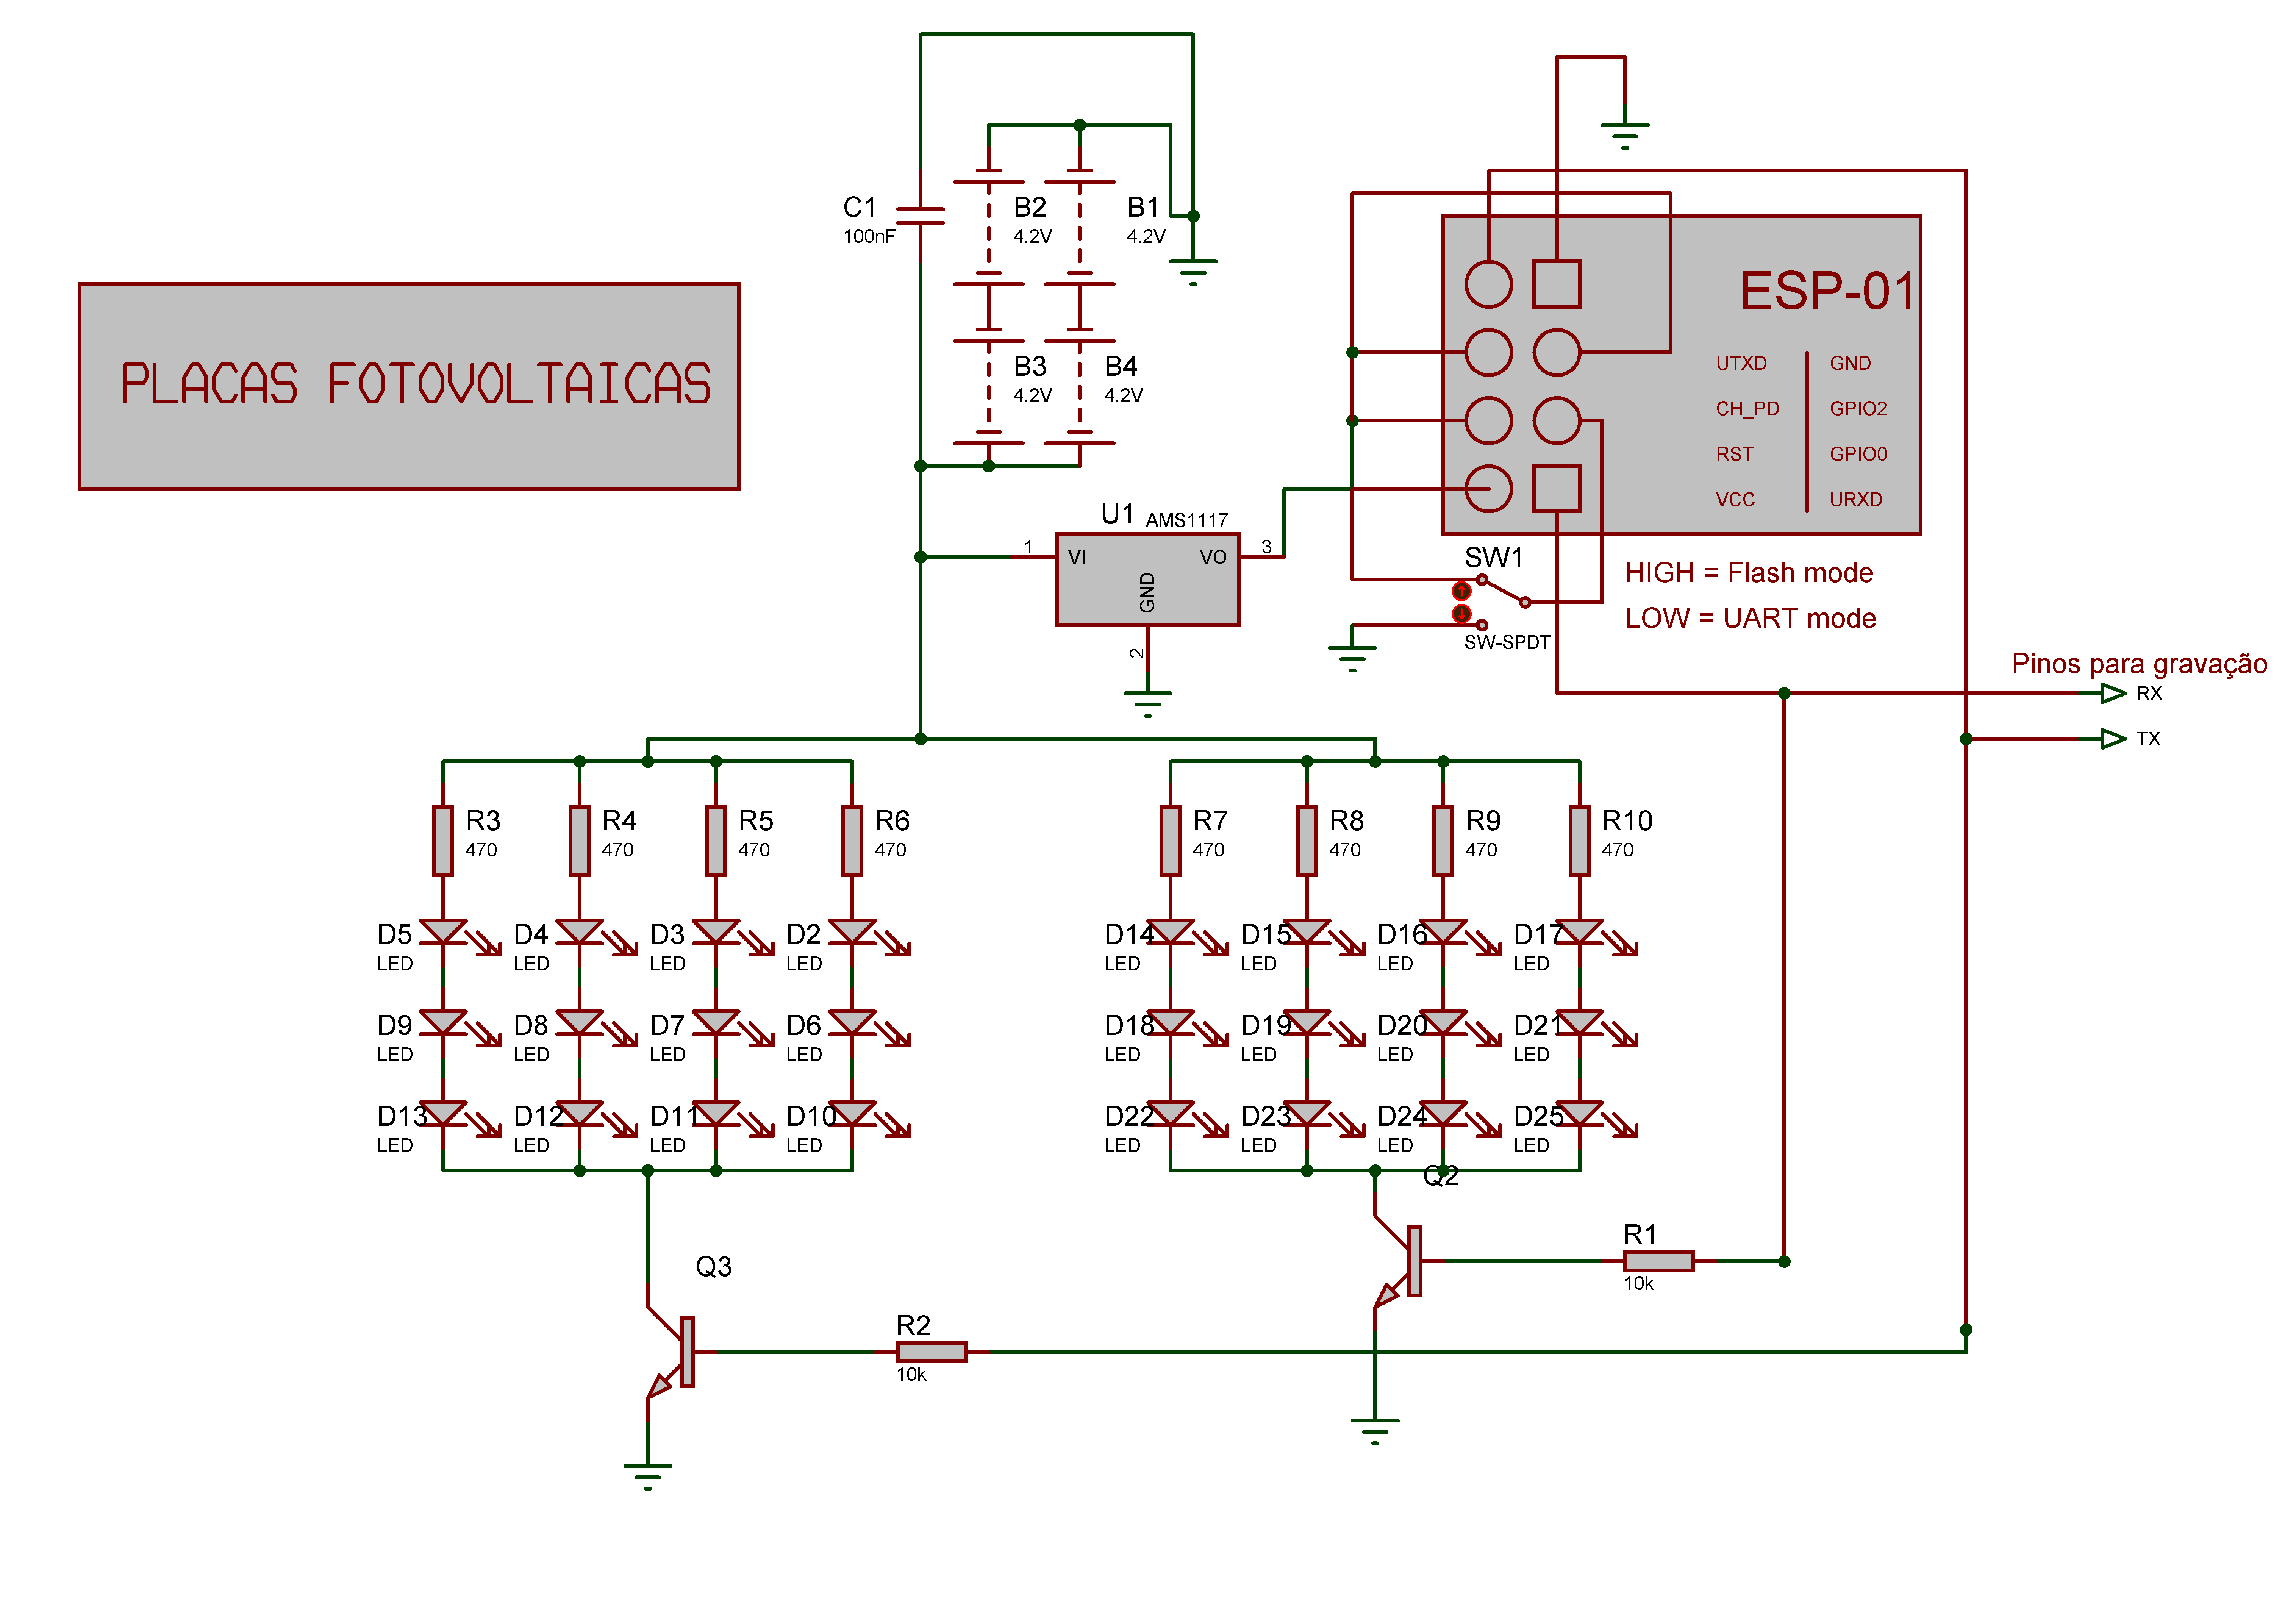
\includegraphics[width=450pt]{images/circuit.png}
    \caption{Esquemático do circuito}
\end{figure}

\section{Alimentação}
\subsection{Regulação}
\section{MCU}
\section{Placas fotovoltaicas}

% ----------------------------------------------------------
% Parte de resultados
% ----------------------------------------------------------
\part{Resultados}

% ---
% Capitulo de revisão de literatura
% ---
\chapter{Lorem ipsum dolor sit amet}

% ---
\section{Aliquam vestibulum fringilla lorem}
% ---

\lipsum[1]

\lipsum[2-3]

% ---
% Finaliza a parte no bookmark do PDF
% para que se inicie o bookmark na raiz
% e adiciona espaço de parte no Sumário
% ---
\phantompart

% ----------------------------------------------------------
% Trabalhos futuros
% ----------------------------------------------------------
\part{Trabalhos futuros}
\chapter{Circuito}

\section{Alimentação}
\subsection{Células fotovoltaicas}

\section{Raspberry pi 3}
\subsection{Web server}
Mais leve

Raspberry por um host contratado

% ---
% Conclusão
% ---
\chapter{Conclusão}
% ---

\lipsum[31-33]

% ----------------------------------------------------------
% ELEMENTOS PÓS-TEXTUAIS
% ----------------------------------------------------------
\postextual

% ----------------------------------------------------------
% Referências bibliográficas
% ----------------------------------------------------------
\bibliography{abntex2-modelo-references}

% ----------------------------------------------------------
% Glossário
% ----------------------------------------------------------
%
% Consulte o manual da classe abntex2 para orientações sobre o glossário.
%
%\glossary

% ----------------------------------------------------------
% Apêndices
% ----------------------------------------------------------

% ---
% Inicia os apêndices
% ---
\begin{apendicesenv}

    % Imprime uma página indicando o início dos apêndices
    \partapendices

    % ----------------------------------------------------------
    \chapter{Quisque libero justo}
    % ----------------------------------------------------------

    \lipsum[50]

    % ----------------------------------------------------------
    \chapter{Nullam elementum urna vel imperdiet sodales elit ipsum pharetra ligula
    ac pretium ante justo a nulla curabitur tristique arcu eu metus}
    % ----------------------------------------------------------
    \lipsum[55-57]

\end{apendicesenv}
% ---


% ----------------------------------------------------------
% Anexos
% ----------------------------------------------------------

% ---
% Inicia os anexos
% ---
\begin{anexosenv}

    % Imprime uma página indicando o início dos anexos
    \partanexos

    % ---
    \chapter{Morbi ultrices rutrum lorem.}
    % ---
    \lipsum[30]

    % ---
    \chapter{Cras non urna sed feugiat cum sociis natoque penatibus et magnis dis
    parturient montes nascetur ridiculus mus}
    % ---

    \lipsum[31]

    % ---
    \chapter{Fusce facilisis lacinia dui}
    % ---

    \lipsum[32]

\end{anexosenv}

%---------------------------------------------------------------------
% INDICE REMISSIVO
%---------------------------------------------------------------------

\phantompart

\printindex

%---------------------------------------------------------------------
% Formulário de Identificação (opcional)
%---------------------------------------------------------------------
\chapter*[Formulário de Identificação]{Formulário de Identificação}
\addcontentsline{toc}{chapter}{Exemplo de Formulário de Identificação}
\label{formulado-identificacao}

Exemplo de Formulário de Identificação, compatível com o Anexo A (informativo)
da ABNT NBR 10719:2015. Este formulário não é um anexo. Conforme definido na
norma, ele é o último elemento pós-textual e opcional do relatório.

\bigskip

\begin{tabular}{|p{9cm}|p{5cm}|}
    \hline
    \multicolumn{2}{|c|}{\textbf{\large Dados do Relatório Técnico e/ou científico}}\\
    \hline
    \multirow{4}{10cm}[24pt]{Título e subtítulo}& Classificação de segurança\\
                                                & \\
                                                \cline{2-2}
                                                & No.\\
                                                & \\

                                                \hline
    Tipo de relatório & Data\\
    \hline
    Título do projeto/programa/plano & No.\\
    \hline
    \multicolumn{2}{|l|}{Autor(es)} \\
    \hline
    \multicolumn{2}{|l|}{Instituição executora e endereço completo} \\
    \hline
    \multicolumn{2}{|l|}{Instituição patrocinadora e endereço completo} \\
    \hline
    \multicolumn{2}{|l|}{Resumo}\\[3cm]
    \hline
    \multicolumn{2}{|l|}{Palavras-chave/descritores}\\
    \hline
    \multicolumn{2}{|l|}{
    Edição \hfill No. de páginas \hfill No. do volume \hfill Nº de classificação \phantom{XXXX}} \\
    \hline
    \multicolumn{2}{|l|}{
    ISSN \hfill \hfill Tiragem \hfill Preço \phantom{XXXXXXXX}} \\
    \hline
    \multicolumn{2}{|l|}{Distribuidor} \\
    \hline
    \multicolumn{2}{|l|}{Observações/notas}\\[3cm]
    \hline
\end{tabular}

   \end{document}
